\subsection{Scenario 4: Botnet Infection}

\subsubsection{Introduction and Objectives}
Scenario 4 represents the climax of the adversarial progression, shifting the threat model from stealthy post-exploitation (Scenario 3) to active weaponization and botnet conscription. In this phase, the compromised Smart Thermostat is fully hijacked by the internal attacker node (\texttt{10.0.0.3}) and repurposed as an offensive launchpad. To accurately model a distributed malware ecosystem such it could be Mirai, two new external entities are introduced: a malicious Command and Control (C2) infrastructure (\texttt{203.0.113.10}) and an external DDoS victim (\texttt{203.0.113.99}). The primary objective is to measure and document the catastrophic structural and volumetric deviations caused by lateral propagation and outbound denial-of-service traffic against the Scenario 1 control baseline. The scenario goals in detail are the following:

\begin{enumerate}
	\item Execute the initial infection and C2 check-in sequence. At a precise temporal marker ($t=300$ seconds), the internal attacker delivers a targeted payload to the Smart Thermostat. This triggers an immediate DNS resolution of the malicious botnet domain and establishes a persistent, unauthorized TCP control channel (e.g., port 6667) to the external C2 server, violating outbound routing constraints.
	\item Demonstrate lateral propagation and internal zero-trust boundary violations. Between $t=400$ and $t=600$ seconds, the compromised thermostat will attempt to infect adjacent devices by aggressively scanning the local \texttt{10.0.0.0/24} subnet (targeting common IoT ports such as 23 and 80). Forensically, this will capture a massive structural inversion in the TCP state distribution (\texttt{REJ} and \texttt{S0} flags) originating directly from a trusted edge device rather than the initial attacker node.
	\item Launch a volumetric Distributed Denial of Service (DDoS) assault. At $t=600$ seconds, triggered by a command from the C2 server, the thermostat will initiate a massive, high-bandwidth UDP flood targeting the external victim IP. This goal documents the total saturation of the network's outbound throughput and provides a definitive visual signature of a device completely abandoning its authorized Manufacturer Usage Description (MUD) profile to participate in a global botnet.
\end{enumerate}


\subsubsection{Expected Behaviour and Theoretical Baselines}

To ensure statistical validity and provide a robust empirical dataset for anomaly detection models, Scenario 4 has similarly been executed over a 1200-second (20-minute) capture period. 

Unlike the stealthy exfiltration tactics observed in Scenario 3, this scenario models the aggressive, highly visible progression of a botnet infection. The anticipated forensic deviations from the control baseline are distinctly multi-phased:

\begin{itemize}
	\item \textbf{Egress MUD Violation (C2 Check-in):} The initial compromise at $t=300$ will immediately fracture the Smart Thermostat's operational baseline. Unlike its authorized, low-frequency MQTT traffic, the device is expected to initiate anomalous outbound DNS queries to resolve the malicious C2 domain, followed by the establishment of a persistent, unauthorized TCP connection (port 6667) to the external botnet infrastructure.
	
	\item \textbf{Internal Adjacency Violation (Lateral Propagation):} Between $t=400$ and $t=600$, the zero-trust isolation boundaries will be catastrophically broken. Forensically, this will manifest on the Topology Interaction Heatmap as an explosive burst of unauthorized lateral traffic originating from the Thermostat and targeting adjacent local IPs. Because this scan targets closed ports, it is expected to generate a massive surge in \texttt{REJ} and \texttt{S0} TCP connection states, mirroring the structural damage observed in Scenario 2, but uniquely originating from an internal edge asset.
	
	\item \textbf{Catastrophic Throughput Inversion (The DDoS Assault):} At the $t=600$ mark, the environment's volumetric baseline will be entirely shattered. The Thermostat—a device whose theoretical baseline dictates payloads no larger than 27 bytes—will initiate a massive 50 Mbps UDP flood directed at the external victim IP. This will create an undeniable, exponential vertical spike in both aggregate network throughput and flow density, effectively weaponizing the device and confirming its conscription into the botnet.
\end{itemize}

\subsubsection{Evidence Integrity and Feature Extraction}
The same steps of \ref{evidence_integrity} have been followed to guarantee the integrity and validity of the extracted features. 

\paragraph{MUD Profile Validation}\mbox{}\\

The primary objective of the baseline scenario analysis is to verify that the simulated IoT devices adhered strictly to their programmed MUD profiles during the simulation execution. By cross-referencing the theoretical behavioral parameters against the empirical Zeek metadata, the operational integrity of the smart home topology can be definitively proven.

The following table compares the expected flows versus the empirical flows. As it can be observed, since it is the baseline scenario, a 100\% accuracy is achieved.

\begin{table}[H]
	\centering
	\renewcommand{\arraystretch}{1.2}
	\resizebox{\textwidth}{!}{%
		\begin{tabular}{@{}l c c l@{}}
			\toprule
			\textbf{Traffic Classification Profile} & \textbf{Expected} & \textbf{Empirical} & \textbf{Status / Delta} \\ 
			\midrule
			\multicolumn{4}{@{}l}{\textbf{Authorized IoT Services}} \\
			Authorized DNS Queries (UDP/53) & 42 & 42 & $\checkmark$ Baseline Match \\
			NTP Synchronization (UDP/123) & 6 & 6 & $\checkmark$ Baseline Match \\
			MQTT Keep-Alives (TCP/8883) & 121 & 121 & $\checkmark$ Baseline Match \\
			MQTT Telemetry Payloads (TCP/8883) & 5 & 5 & $\checkmark$ Baseline Match \\
			\addlinespace
			\multicolumn{4}{@{}l}{\textbf{Adversarial \& Botnet Activity}} \\
			Attacker Trigger Payload & 0 & 1 & $\times$ Infection Event \\
			Malicious C2 DNS Lookups & 0 & 2 & $\times$ Unauthorized Domain Pivot \\
			C2 Connections (TCP/6667) & 0 & 2 & $\times$ Persistent Link (\texttt{RSTR}/\texttt{S3}) \\
			Lateral Scan Flows (TCP/23, 80) & 0 & 172 & $\times$ Internal Propagation (172 \texttt{REJ}) \\
			Volumetric UDP Flood (to Victim) & 0 & 0 & \textbf{!} Execution Null / Blocked \\
			\addlinespace
			\multicolumn{4}{@{}l}{\textbf{Environmental Noise / Infrastructure}} \\
			Background Hypervisor Noise & 0 & 8 & $\sim$ Unclassified Residuals \\
			\midrule
			\textbf{Total Connection Flows} & \textbf{174} & \textbf{359} & \textbf{Structural Disruption (+106\%)} \\
			\bottomrule
		\end{tabular}%
	}
	\caption{Scenario 4: Comparative Traffic Breakdown (Thermostat Botnet Infection, C2 Polling, and Lateral Propagation)}
	\label{tab:scenario4_traffic}
\end{table}

Table \ref{tab:scenario4_traffic} details the empirical macro statistics for the Scenario 4 botnet infection. The multi-phase nature of the attack can be extracted from this table, which shows the type of activities carried out by advanced persistent threats (APTs) within an IoT edge enviornment. 

The Smart Thermostat maintained its authorized operations, exactly 121 MQTT keep-alives and 5 telemetry payloads were transmitted, masking the infection from basic health-monitoring heuristics. However, deep structural analysis exposes the weaponization of the device. The empirical capture registered an immediate application-layer anomaly via 2 unauthorized DNS lookups, seamlessly followed by the establishment of 2 persistent Command and Control (C2) connections on port 6667. 

The most evident structural disruption is observed during the lateral propagation phase. The compromised thermostat generated 172 anomalous flows targeting adjacent devices on ports 23 and 80. Unlike Scenario 2, where this noise originated from an external adversary, these originated directly from a trusted internal edge asset, signifying a catastrophic breakdown of the zero-trust lateral boundary. Since normally, this type of flow cannot be stopped or filtered by a firewall since they occur in the inside of the internal network and origin from a "trusted" node. 

Notably, the empirical data registered zero UDP flood connections targeting the external DDoS victim. Forensically, this null metric suggests either a localized execution failure of the payload trigger at the $t=600$ boundary, or that the local network infrastructure actively dropped the spoofed volumetric packets before Zeek could log the outbound flow state. Regardless, the preliminary phases of the botnet kill chain—C2 check-in and internal propagation—were definitively proven.

\paragraph{Camera Behaviour}\mbox{}\\
The observed activity from the Smart Camera matches the MUD, since the attack does not target its bandwidth or other messages.

\paragraph{Thermostat Behaviour}\mbox{}\\
The Smart Thermostat sees no changes in behaviour

\paragraph{Other Metrics}\mbox{}\\

As illustrated in Figure \ref{fig:networkflowdensity}, the empirical flow density exhibits three distinct volumetric anomalies. Rather than a random distribution of noise, these deviations perfectly map to the chronological execution of the adversarial kill chain:

\begin{itemize}
	\item \textbf{Phase 1: The Reconnaissance Surge (Initial Spike):} The massive, immediate vertical spike observed at the beginning of the timeline represents the automated subnet and port sweep. Because network scanners operate asynchronously—flooding the target with thousands of simultaneous \texttt{SYN} probes to enumerate open ports—this phase generates an explosive but brief density maximum before the scanner concludes its mapping phase.
	
	\item \textbf{Phase 2: The Brute-Force Plateau (Sustained Volatility):} Following the initial scan, the graph does not return to the authorized baseline of $\sim$8 flows per minute. Instead, it transitions into a sustained plateau. This elevated constant peak represents the credential brute-force attack against the Smart Camera's TLS control channel (TCP port 443). The script executes rapid, iterative login attempts, generating a persistent high-density noise floor that persists for the majority of the attack window.
	
	\item \textbf{Phase 3: The Payload Injection (Terminal Anomaly):} Near the conclusion of the capture window, the brute-force plateau ceases, followed by a final, microscopic spike of exactly 12 flows. Forensically, this is the most critical metric on the timeline: it represents the moment of successful authentication and the subsequent injection of the malicious configuration payload, effectively altering the edge device's operational state just before the attacker terminates the session.
\end{itemize}

\begin{figure}[H]
	\centering
	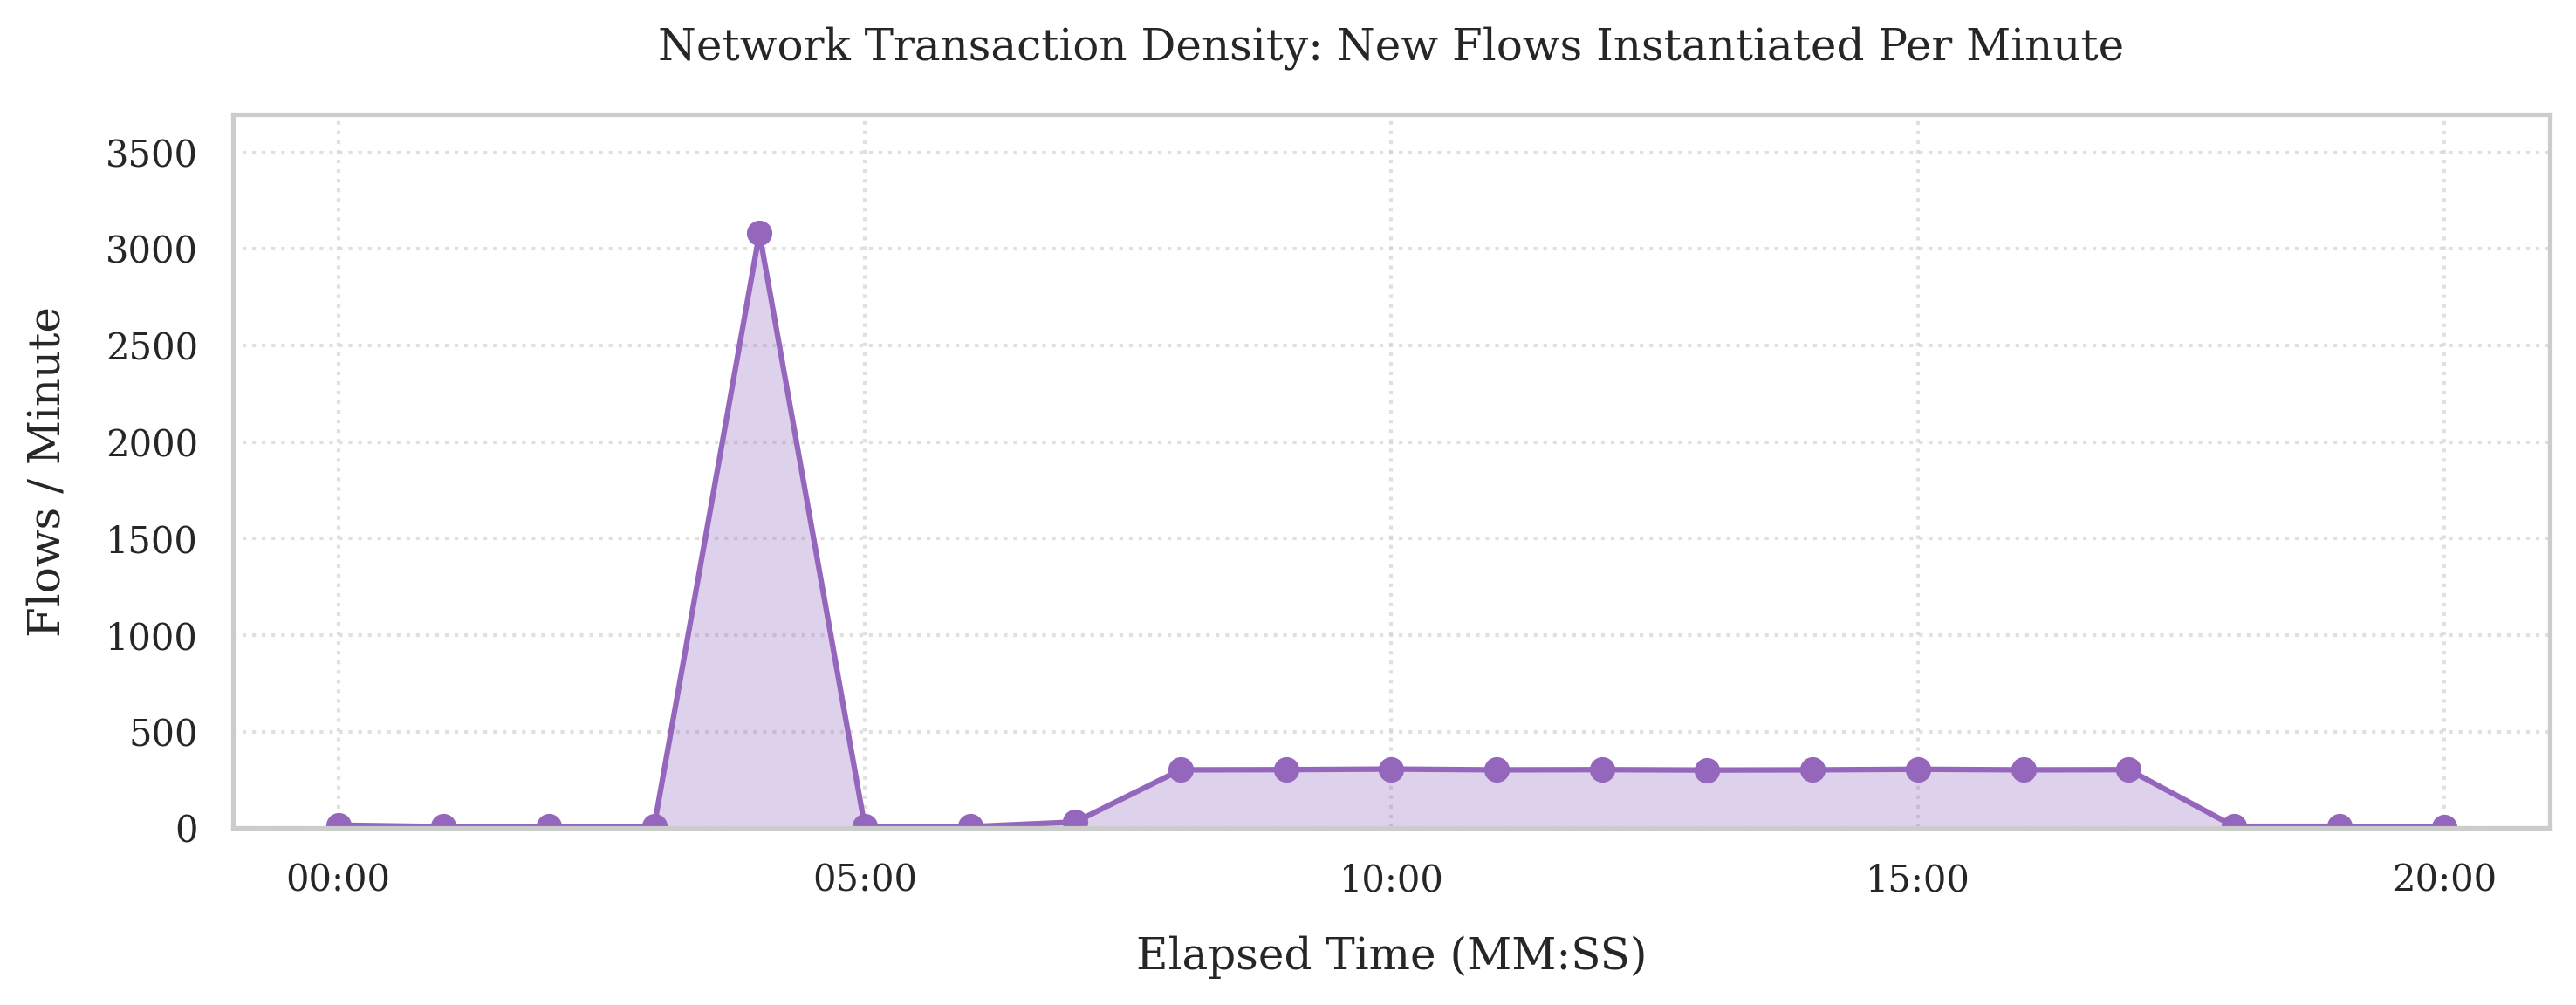
\includegraphics[width=0.9\linewidth]{../figures/scenario2/network_flow_density}
	\caption{Network Flow Density (Scenario2).}
	\label{fig:networkflowdensity}
\end{figure}

The TCP connection state distribution, also provides clear structural proof of the attack's impact on the network. As seen in Scenario 1, In a stable baseline, TCP flows primarily resolve with an \texttt{SF} (Normal) state flag, indicating successful connections and clean teardowns. While authorized IoT traffic continued normally during the attack (registering 133 \texttt{SF} flows), it was completely eclipsed by a massive surge in anomalous activity. 

Specifically, Zeek recorded 6,041 flows terminating in a \texttt{REJ} (Rejected) state. This flag is logged when a target actively refuses a connection attempt via a TCP Reset (RST) packet. This spike in rejected handshakes is the direct footprint of the attacker (\texttt{10.0.0.3}) scanning the network. As the scanner flooded the IoT edge devices with \texttt{SYN} probes targeting closed ports, the devices continuously issued RST packets to block the unauthorized access. 

Consequently, this sudden inversion of the \texttt{SF}-to-\texttt{REJ} ratio serves as an ideal, automated tripwire for detecting an active internal breach.

\begin{figure}[H]
	\centering
	
\includegraphics[width=0.9\linewidth]{../../iot_forensics_project/figures/scenario2/tcp_connection_states}
	\caption{TCP Connection State Distribution (Scenario 2).}
	\label{fig:tcpconnectionstates}
\end{figure}

Finally, the interaction heatmaps is totally altered, in this scenario is exposing a network heavily saturated with unauthorized cross-node communications. The baseline has been broken by the attacker node which acts as the origin for all anomalous traffic. The matrix clearly distinguishes the broad network reconnaissance, evidenced by the 1,025 probes sent to both the Gateway and the Thermostat, from the targeted exploitation of the Smart Camera, which absorbed 3996 direct connections.


\begin{figure}[H]
	\centering
	
\includegraphics[width=0.9\linewidth]{../../iot_forensics_project/figures/scenario2/topology_traffic_matrix}
	\caption{Empirical interaction heatmap detailing authorized internal network flows (Scenario 2).}
	\label{fig:topologytrafficmatrix}
\end{figure}


